\documentclass{article}

% Environment setup

\usepackage[
    margin=1in
]{geometry} %geometry (sets margin) and other useful packages 
\setlength{\oddsidemargin}{.25in}
\setlength{\evensidemargin}{.25in}
\setlength{\textwidth}{6in}
\setlength{\topmargin}{-0.4in}
\setlength{\textheight}{8.5in}
\setlength{\parindent}{0em}
\setlength{\parskip}{.75em}

\usepackage{graphicx}
\usepackage{grffile}  % support extra dots in filenames
\usepackage{fancyref}
\usepackage[labelfont=bf]{caption}
\usepackage{subcaption}


\title{\textbf{CS 4641:} Supervised Learning}
\author{Bradley Reardon}
\date{February 10, 2019}

\begin{document}
    \maketitle

    \section{Introduction}
    The purpose of this assignment is to evaluate various supervised learning techniques in the context of two classification algorithms. We will focus on analyzing and adjusting five learning algorithms using two publically-available data sets, through cross-validation and hyperparameter adjustments. Then, we can use our adjusted models to compare supervised learning techniques in the context of each of our classification algorithms.

    \subsection{Collaboration disclosure}
    I collaborated on the programming portion of this assignment with Nikolai Vorobiev in order to produce a code-base capable of using scikit-learn to effectively evaluate the given data sets. Though the code we used to run analysis on the algorithms is the same, this analysis is wholly my own.

    \section{Classification algorithms}
    For the purposes of this report, data sets were obtained from the UCI Machine Learning Repository. Each data set downloaded was processed with a custom script in the corresponding folder, \textbf{process.py}, which randomly separated the data into an 80\% training data and 20\% test data split using the \textbf{train\_test\_split} function from scikit-learn. The split data was then serialized using Python's \textbf{pickle} module into \textbf{.dataset} files, to ensure that the training and test sets remained constant for evaluation.

    For the purposes of this assignment, cross-validation scoring of the various algorithms for each classification problem will be shown as the average score of 5-fold cross validation.

    \subsection{Car data set}
    The Car Evaluation Database was created in June, 1997 by Marko Bohanec. It contains 1728 instances and six attributes. The purpose of this database is to attempt to classify a car as an unacceptable, acceptable, good, or very good choice based on factors including cost of ownership, comfort, and safety. Full details about the data set can be found at the source link below.

    The problem at hand for this dataset is determining the acceptability for a car purchase based on the aforementioned attributes. Because this dataset notes that the instances in the data set completely cover the attribute space, this data set is interesting in particular due to its usefulness in comparing the optimization of different supervised learning algorithms. Note that this specific data set contains only categorical attributes. As scikit-learn does not support non-continuous variables, a one-hot encoder was used to re-encode categorical features into multiple dimensions.

    \textbf{Source:} https://archive.ics.uci.edu/ml/datasets/car+evaluation

    \subsection{Breast Cancer Wisconsin data set}
    The Breast Cancer Wisconsin data set was donated to the UCI Machine Learning Repository in 1992, and contains data from one doctor's clinical cases, gathered from January 1989 to November 1991. In total, there are 699 instances signifying information about breast tumors such as clump thickness, uniformity in shape and size, and other screening factors. Data points are identified by two classes -- benign or malignant. The features of the data points are encoded as 9 continuous attributes rating the screening factor from 1 to 10.

    This data set contains unknowns in the form of question marks in the data. To deal with this, missing values were imputed, calculating missing data points based on the mean of other points in the specific column of the missing attribute. 

    The problem at hand for this dataset is determining whether a tumor is benign or malignant based on tumor screening characteristics identified in the data set.

    \textbf{Source:} https://archive.ics.uci.edu/ml/datasets/Breast+Cancer+Wisconsin+\%28Original\%29

    \section{Decision trees with pruning}

    \subsection{Parameter selection}
    To begin evaluating the decision tree algorithm, hyperparameter selection was essential to tuning the algorithms to each data set. Both the car and cancer datasets were evaluated with the GINI index criterion as well as the entropy criterion. The two criterion had no discernible differences in training results, so as a result, GINI was selected for the decision tree classifier on both sets, as it allows us to avoid a logarithmic calculation, saving compute time.

    The next parameters that needed tuning were the pruning parameters included in the scikit-learn decision tree classifier. Namely, the max depth of the tree, as well as the minimum samples per leaf, were tuned to fit each data set.

    For the car data set, parameter selection showed that a lower-depth tree had much lower accuracy, likely due to the fact that the dataset had instances covering the entire attribute space. As a result, a max depth of 9 nodes was selected for the car data set, with a minimum number of 5 samples occurring at each leaf node to minimize the amount of information loss.

    The cancer data set, on the other hand, responded much better to more aggressive pruning. The pruned decision tree classifier responded to the data with the best F1 score with a max depth of 5 nodes, and a minimum number of 10 samples occurring at each leaf.

    \subsection{Performance}
    Performance of the tuned classifier for each data set was measured with both wall clock time for fitting the model with the training data, as well as making a prediction with the test data. For the breast cancer data set, pruning resulted in both higher precision and accuracy, with a performance gain during prediction over a non-pruned decision tree (from 0.801ms to 0.479ms). However, the classifier took 0.57 seconds longer to train with pruning enabled (no pruning: 2.38s, pruning: 2.95s). For this data set, with the determined parameters was successful.

    However, the car data set showed different results with pruning enabled. There was no significant change in either the precision or accuracy measures. The car data set's decision tree classifier took 11.51 seconds to fit without pruning, however with pruning this was reduced to 7.35s with pruning. Prediction runtime for the pruned tree was only slightly longer than the unpruned tree. Due to the completeness of the data, pruning is likely not necessary for this dataset without further tuning.

    Learning curves for the data sets, with and without pruning enabled, can be found in \Fref{fig:dt-learning}.

    \begin{figure}[htb]
    \centering

    \begin{subfigure}{0.5\textwidth}
      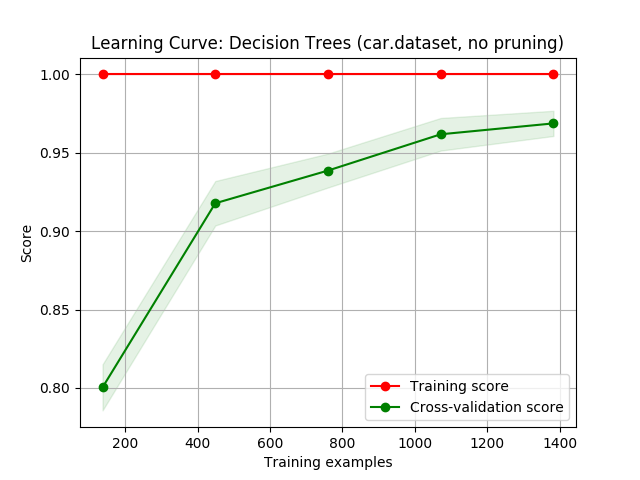
\includegraphics[width=\linewidth]{out/decision_tree_pruning/car-noprune-learning.png}
      \caption{Car data set, no pruning}
      \label{fig:dt-learning-1}
    \end{subfigure}\hfil
    \begin{subfigure}{0.5\textwidth}
      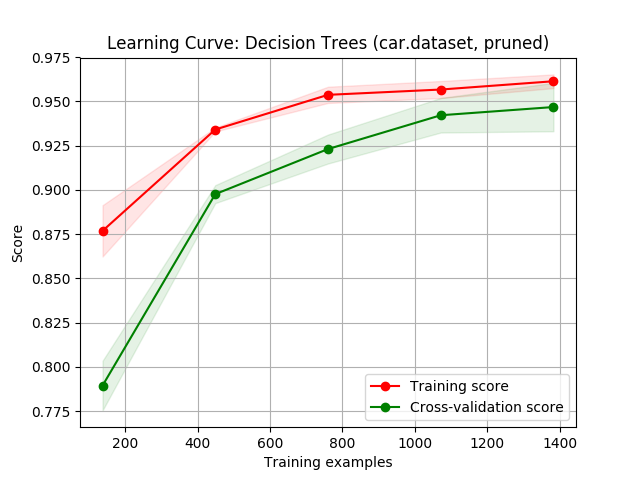
\includegraphics[width=\linewidth]{out/decision_tree_pruning/car-prune-learning.png}
      \caption{Car data set, with pruning}
      \label{fig:dt-learning-2}
    \end{subfigure}

    \medskip

    \begin{subfigure}{0.5\textwidth}
      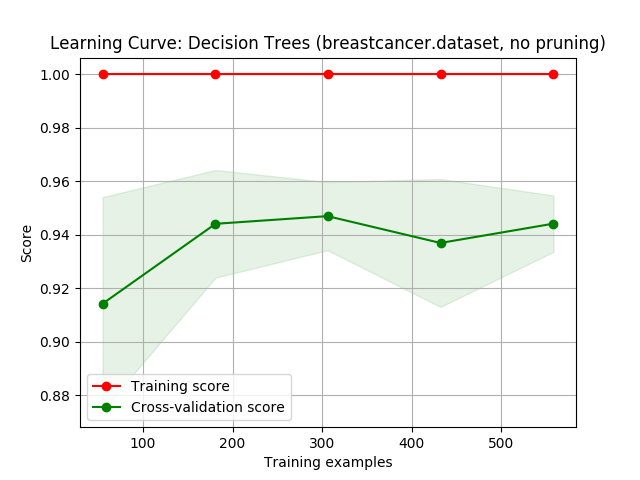
\includegraphics[width=\linewidth]{out/decision_tree_pruning/breastcancer-noprune-learning.png}
      \caption{Breast cancer data set, no pruning}
      \label{fig:dt-learning-3}
    \end{subfigure}\hfil
    \begin{subfigure}{0.5\textwidth}
      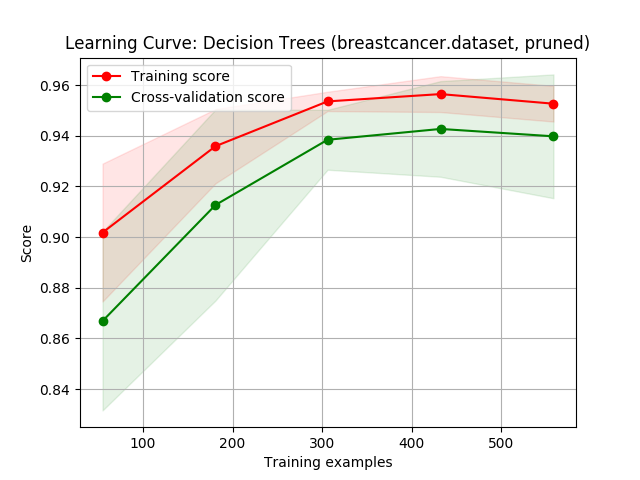
\includegraphics[width=\linewidth]{out/decision_tree_pruning/breastcancer-prune-learning.png}
      \caption{Breast cancer data set, with pruning}
      \label{fig:dt-learning-4}
    \end{subfigure}

    \caption{Learning curves for the car and breast cancer data sets using a decision tree classifier, with and without pruning.}
    \label{fig:dt-learning}
    \end{figure}

    \section{Boosting}
    We will next evaluate the AdaBoost boosting algorithm included in scikit-learn, using the pruned decision trees from the previous section as base estimators for the algorithm.

    \subsection{Parameter selection}
    For the AdaBoost algorithm, there were three main parameters that needed to be determined. The graphs in \Fref{fig:boosting-param} were used to determine the proper learning rate, number of estimators, and algorithm for both data sets.

    \begin{itemize}
        \item \textbf{n\_estimators:} the max number of classifiers (decision trees) to fit to the AdaBoost classifier
        \item \textbf{learning\_rate:} shrinks the contribution of each classifier by this amount
        \item \textbf{algorithm:} scikit-learn supports two algorithms derived from AdaBoost -- AdaBoost-SAMME and AdaBoost-SAMME.R. SAMME is usually used for discrete values, whereas SAMME.R is used for real/continuous values. 
    \end{itemize}

    The graphs in \Fref{fig:boosting-param} show that the car data generally has lower error with the SAMME algorithm, whereas the breast cancer data leads to lower error when fit with the SAMME.R algorithm. For both sets, the error was generally minimized with a learning rate of 1.0, so that rate was selected for both classifiers.

    \begin{figure}[htb]
    \centering

    \begin{subfigure}{0.33\textwidth}
      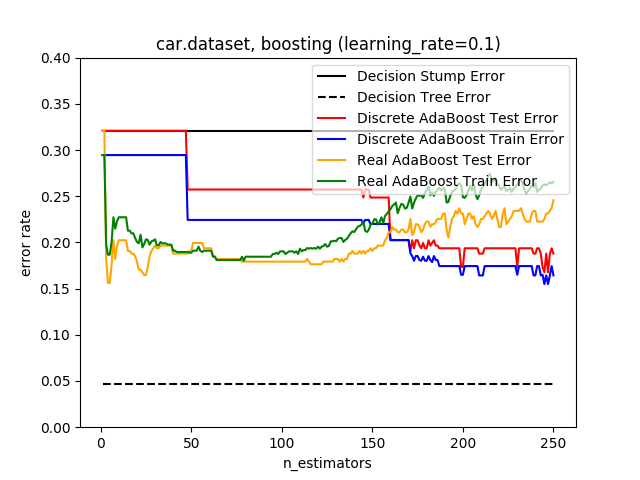
\includegraphics[width=\linewidth]{out/boosting/car-error-lrate-0.1.png}
      \caption{Car data, l\_rate=0.1}
      \label{fig:boosting-param-1}
    \end{subfigure}\hfil
    \begin{subfigure}{0.33\textwidth}
      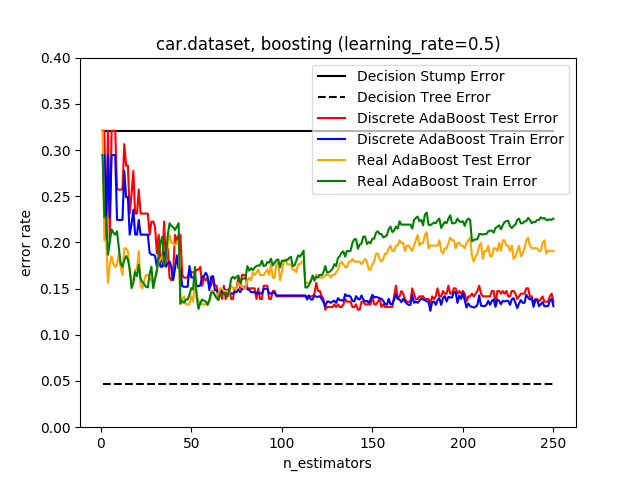
\includegraphics[width=\linewidth]{out/boosting/car-error-lrate-0.5.png}
      \caption{Car data, l\_rate=0.5}
      \label{fig:boosting-param-2}
    \end{subfigure}\hfil
    \begin{subfigure}{0.33\textwidth}
      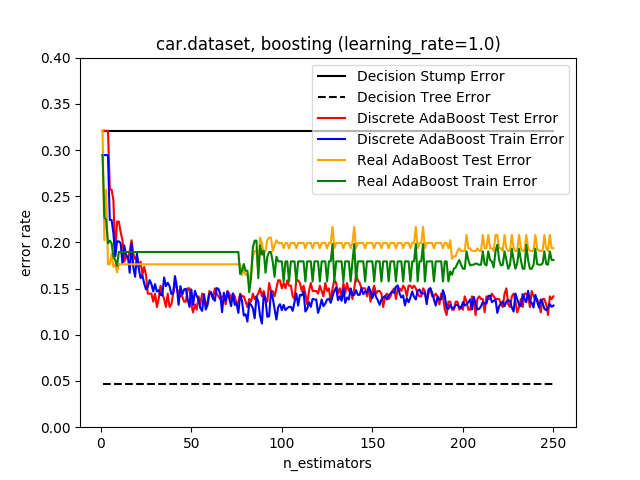
\includegraphics[width=\linewidth]{out/boosting/car-error-lrate-1.0.png}
      \caption{Car data, l\_rate=1.0}
      \label{fig:boosting-param-3}
    \end{subfigure}

    \medskip

    \begin{subfigure}{0.33\textwidth}
      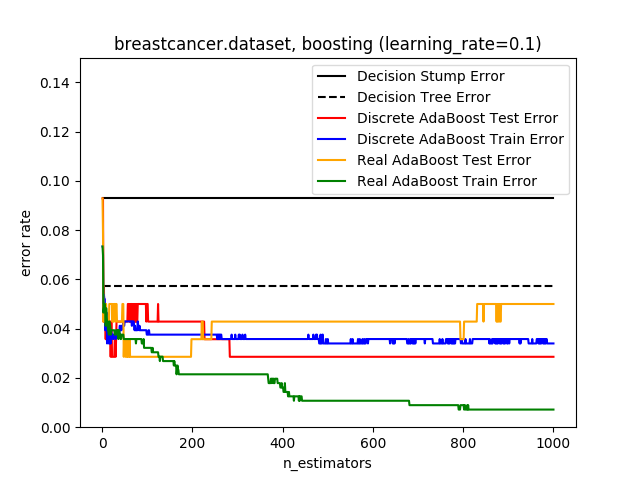
\includegraphics[width=\linewidth]{out/boosting/breastcancer-error-lrate-0.1.png}
      \caption{Cancer data, l\_rate=0.1}
      \label{fig:boosting-param-4}
    \end{subfigure}\hfil
    \begin{subfigure}{0.33\textwidth}
      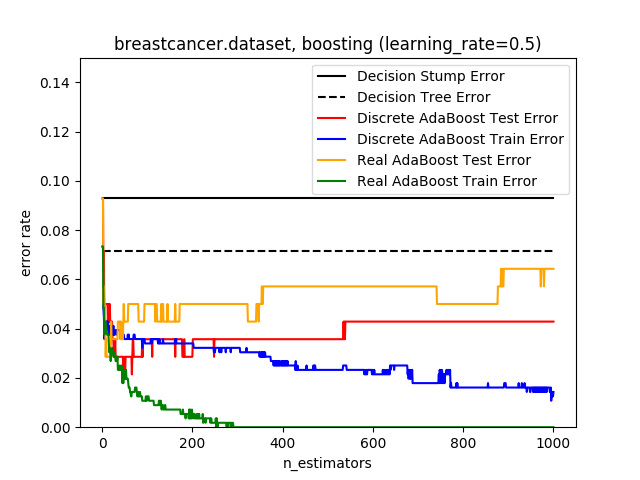
\includegraphics[width=\linewidth]{out/boosting/breastcancer-error-lrate-0.5.png}
      \caption{Cancer data, l\_rate=0.5}
      \label{fig:boosting-param-5}
    \end{subfigure}\hfil
    \begin{subfigure}{0.33\textwidth}
      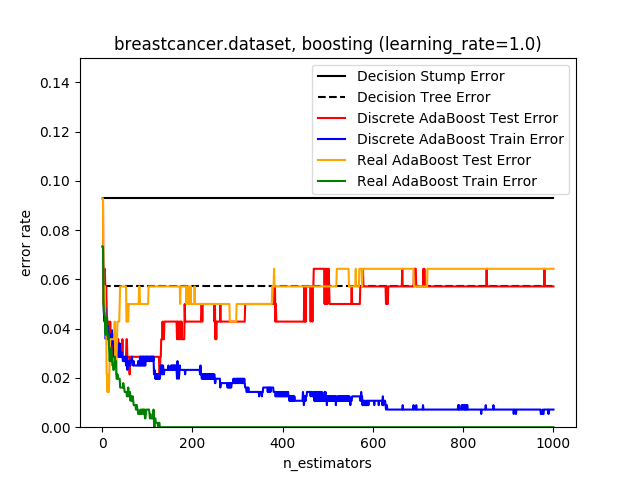
\includegraphics[width=\linewidth]{out/boosting/breastcancer-error-lrate-1.0.png}
      \caption{Cancer data, l\_rate=1.0}
      \label{fig:boosting-param-6}
    \end{subfigure}

    \caption{Selecting a learning rate and number of estimators for the AdaBoot algorithm, using the car and breast cancer sets.}
    \label{fig:boosting-param}
    \end{figure}

    The number of estimators was also determined from the error graphs in \Fref{fig:boosting-param}. The lowest number of estimators where error for the chosen algorithm was minimized was chosen as the number of estimators for each data set. For the car data set, this was approximately 100 estimators, while the cancer data set performed best with around 200 estimators.

    \subsection{Performance}
    \Fref{fig:boosting-perf} shows the learning curves for the car and data set pruned decision tree classifiers before and after applying boosting. Boosting provided a tangible benefit in accuracy and precision for both data sets after proper parameter selection. With the chosen parameters, the car data set and the cancer data set both showed better cross-validation scores with boosting than over the standard pruned decision tree classifiers in the previous section.

    \begin{figure}[htb]
    \centering

    \begin{subfigure}{0.5\textwidth}
      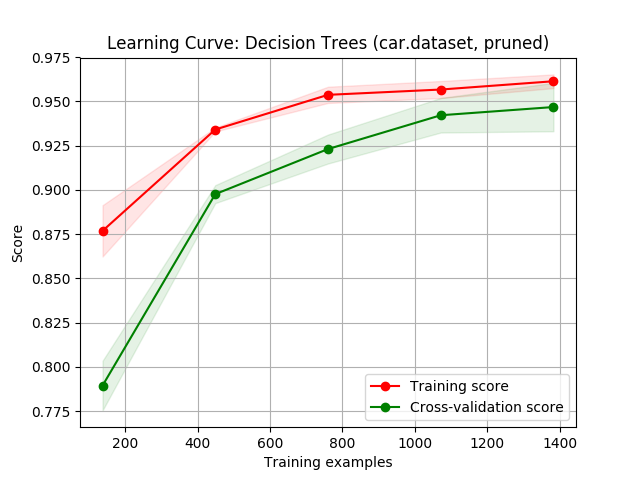
\includegraphics[width=\linewidth]{out/decision_tree_pruning/car-prune-learning.png}
      \caption{Car data, pruning, no boosting}
      \label{fig:boosting-perf-1}
    \end{subfigure}\hfil
    \begin{subfigure}{0.5\textwidth}
      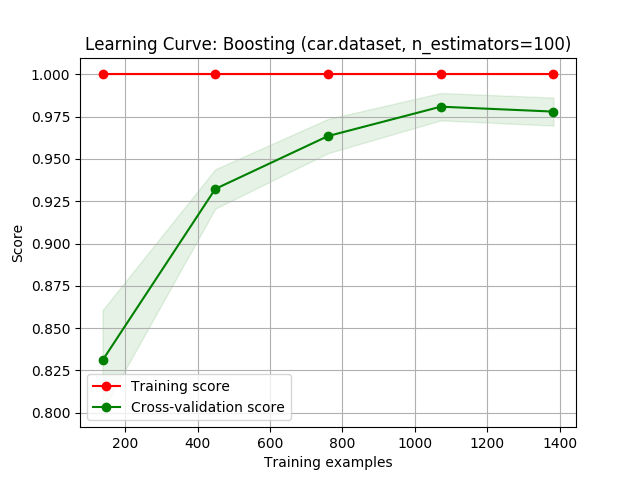
\includegraphics[width=\linewidth]{out/boosting/car-estimators-100.png}
      \caption{Car data, pruning, with boosting}
      \label{fig:boosting-perf-2}
    \end{subfigure}

    \medskip

    \begin{subfigure}{0.5\textwidth}
      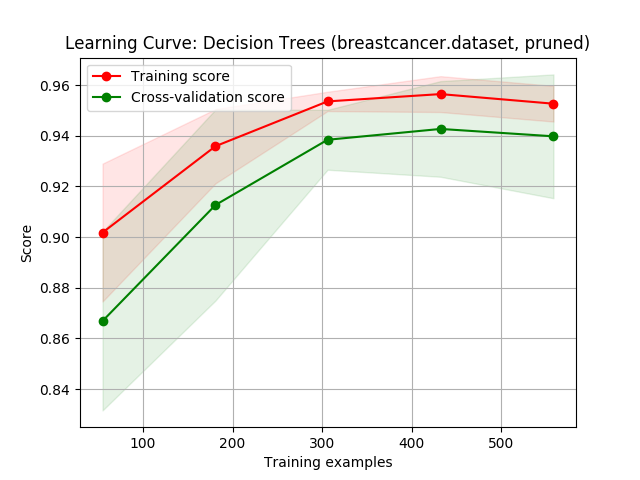
\includegraphics[width=\linewidth]{out/decision_tree_pruning/breastcancer-prune-learning.png}
      \caption{Breast cancer data, pruning, no boosting}
      \label{fig:boosting-perf-3}
    \end{subfigure}\hfil
    \begin{subfigure}{0.5\textwidth}
      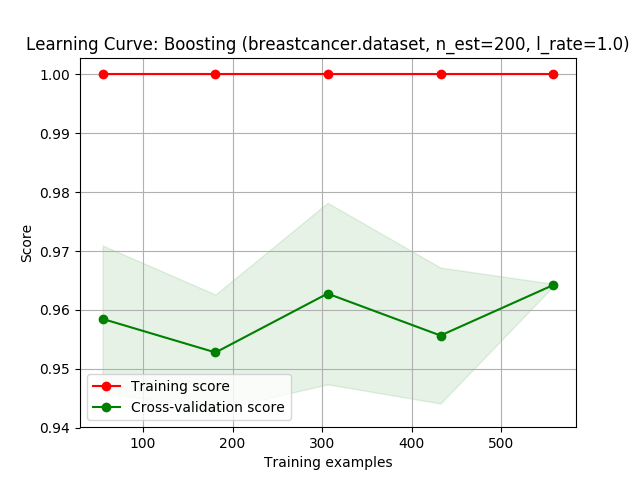
\includegraphics[width=\linewidth]{out/boosting/breastcancer-estimators-200.png}
      \caption{Breast cancer data, pruning, with boosting}
      \label{fig:boosting-perf-4}
    \end{subfigure}

    \caption{Learning curves for the car and cancer data sets, with and without boosting on a pruned decision tree.}
    \label{fig:boosting-perf}
    \end{figure}

    However, this increase in accuracy and precision for both data sets does come at the cost of extra wall clock time during both the fit and predict phases of testing. Due to the nature of the AdaBoost algorithm, fit and prediction times increase with some linearity to the number of estimators used to fit the classifier. This increase in time represented approximate 70-fold and 61-fold increases in fit times for the cancer and car data sets respectively. Similar slow downs resulted in prediction using the boosting algorithm over a standard pruned decision tree.

    Therefore, boosting does increase the accuracy and precision for both models, however at the cost of slowing down fit and classification times across the board.

    \section{Neural networks}
    TODO

    \section{Support vector machines}
    

    \subsection{Performance}

    Learning curves for the car and breast cancer data sets can be found in \Fref{fig:svm-learning}.

    TODO kernel params?

    \begin{figure}[htb]
    \centering

    \begin{subfigure}{0.33\textwidth}
      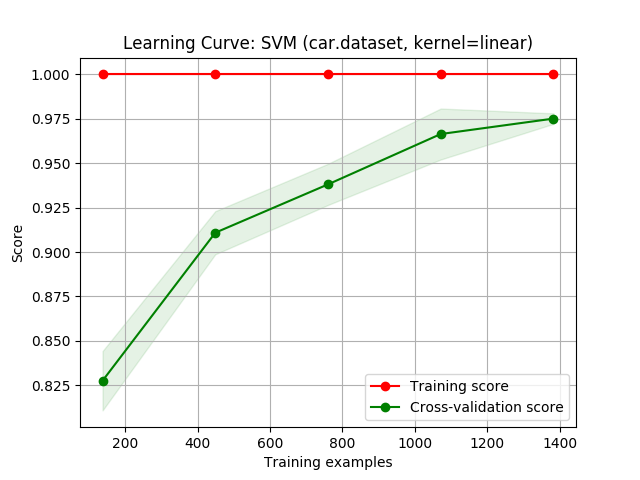
\includegraphics[width=\linewidth]{out/svm/car-kernel-linear.png}
      \caption{Car data, linear kernel}
      \label{fig:svm-learning-1}
    \end{subfigure}\hfil
    \begin{subfigure}{0.33\textwidth}
      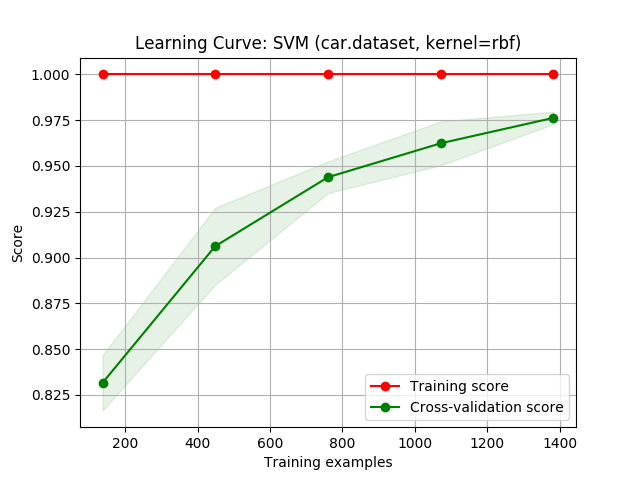
\includegraphics[width=\linewidth]{out/svm/car-kernel-rbf.png}
      \caption{Car data, RBF kernel}
      \label{fig:svm-learning-2}
    \end{subfigure}\hfil
    \begin{subfigure}{0.33\textwidth}
      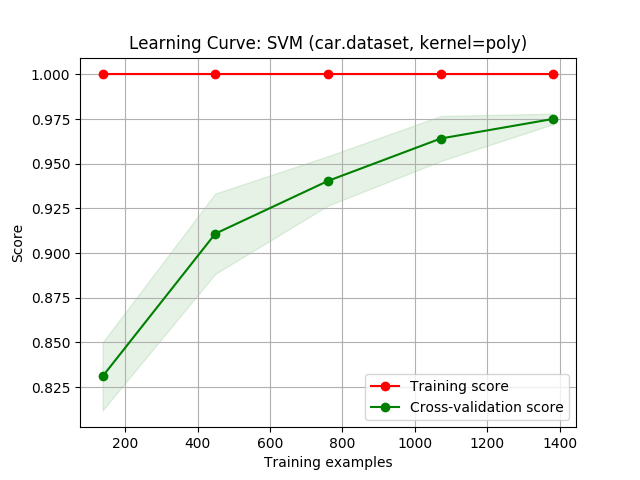
\includegraphics[width=\linewidth]{out/svm/car-kernel-poly.png}
      \caption{Car data, poly kernel}
      \label{fig:svm-learning-3}
    \end{subfigure}

    \medskip

    \begin{subfigure}{0.33\textwidth}
      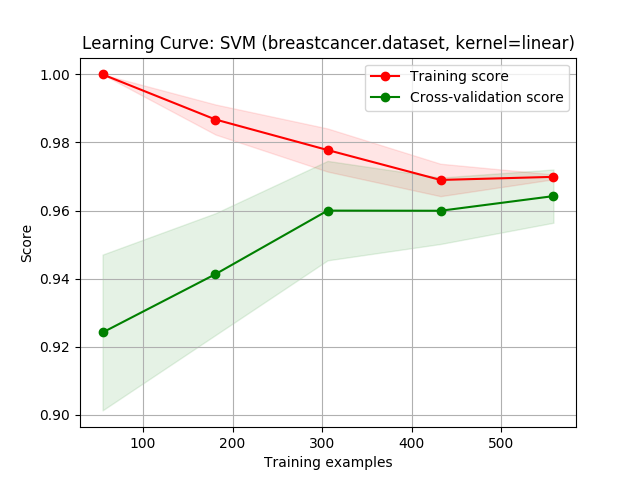
\includegraphics[width=\linewidth]{out/svm/breastcancer-kernel-linear.png}
      \caption{Breast cancer, linear kernel}
      \label{fig:svm-learning-4}
    \end{subfigure}\hfil
    \begin{subfigure}{0.33\textwidth}
      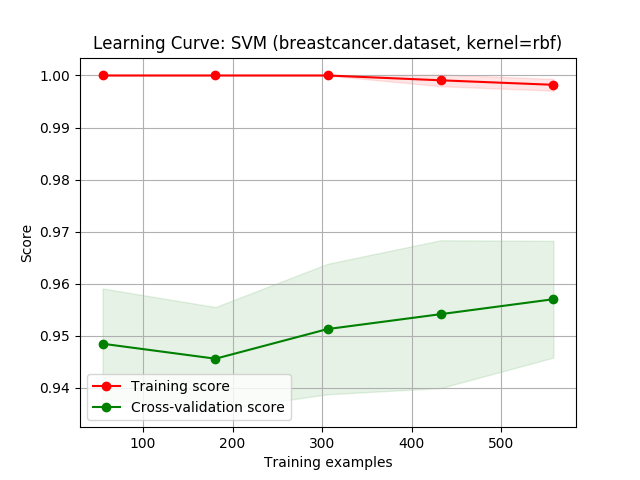
\includegraphics[width=\linewidth]{out/svm/breastcancer-kernel-rbf.png}
      \caption{Breast cancer, RBF kernel}
      \label{fig:svm-learning-5}
    \end{subfigure}\hfil
    \begin{subfigure}{0.33\textwidth}
      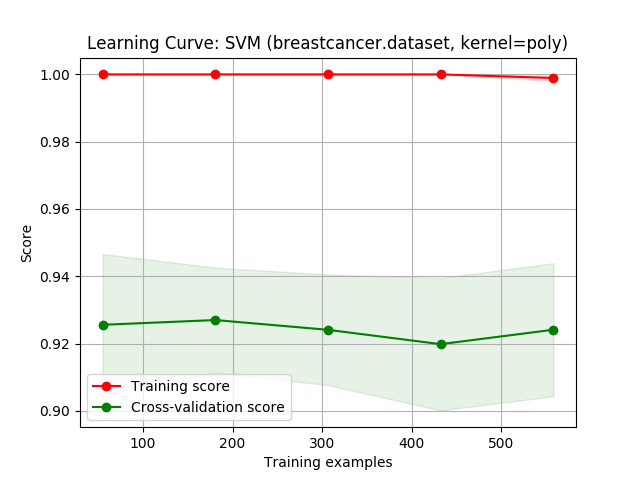
\includegraphics[width=\linewidth]{out/svm/breastcancer-kernel-poly.png}
      \caption{Breast cancer, poly kernel}
      \label{fig:svm-learning-6}
    \end{subfigure}

    \caption{Learning curves for the car and breast cancer data sets using an SVM classifier, with linear, RBF, and poly kernels.}
    \label{fig:svm-learning}
    \end{figure}

    \section{$k$-nearest neighbors}
    TODO

    \subsection{Parameter selection}
    car k=11
    cancer k=5

    Lowest k with highest cross-validation

    TODO \Fref{fig:knn-param}

    \begin{figure}[htb]
    \centering

    \begin{subfigure}{0.5\textwidth}
      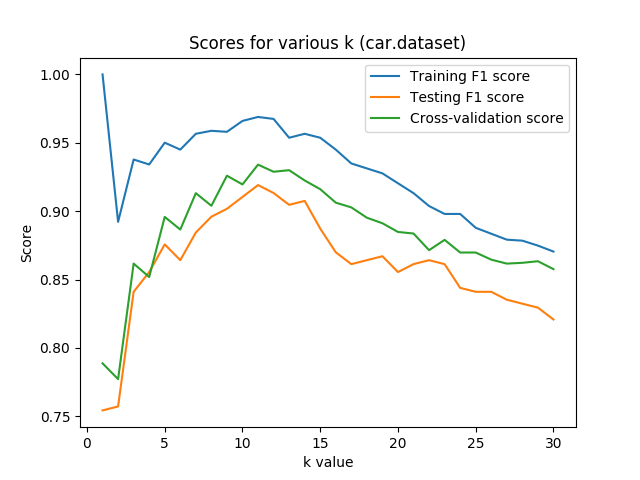
\includegraphics[width=\linewidth]{out/knn/car-k-testing.png}
      \caption{Car data set}
      \label{fig:knn-param-1}
    \end{subfigure}\hfil
    \begin{subfigure}{0.5\textwidth}
      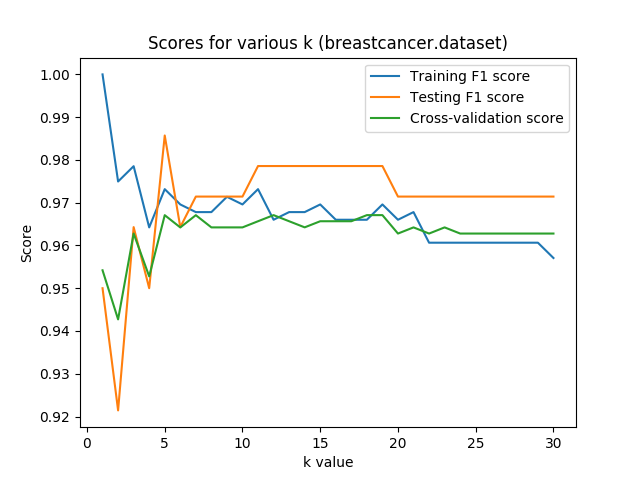
\includegraphics[width=\linewidth]{out/knn/breastcancer-k-testing.png}
      \caption{Breast cancer data set}
      \label{fig:knn-param-2}
    \end{subfigure}

    \caption{Testing $k$-nearest neighbors with various values of $k$.}
    \label{fig:knn-param}
    \end{figure}

    \subsection{Performance}

    TODO \Fref{fig:knn-learning}

    \begin{figure}[htb]
    \centering

    \begin{subfigure}{0.5\textwidth}
      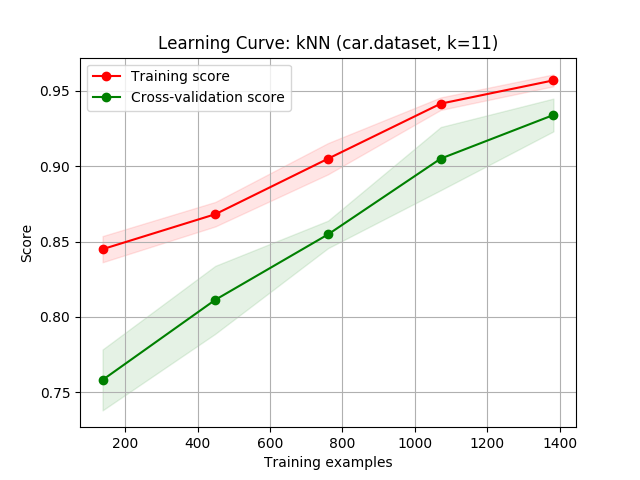
\includegraphics[width=\linewidth]{out/knn/car-k-11.png}
      \caption{Car data set, $k=11$}
      \label{fig:knn-learning-1}
    \end{subfigure}\hfil
    \begin{subfigure}{0.5\textwidth}
      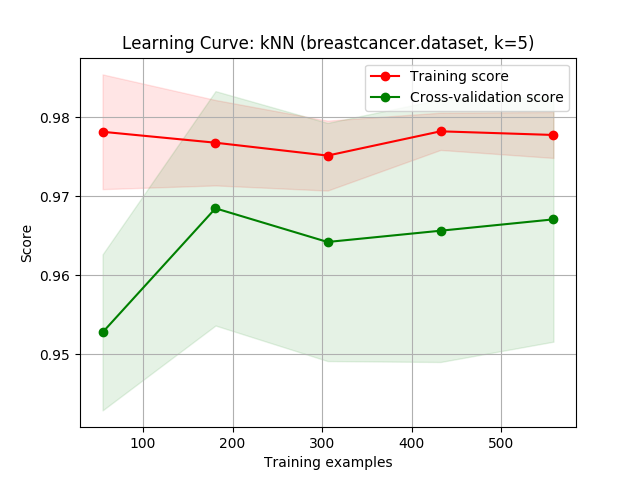
\includegraphics[width=\linewidth]{out/knn/breastcancer-k-5.png}
      \caption{Breast cancer data set, $k=5$}
      \label{fig:knn-learning-2}
    \end{subfigure}

    \caption{Learning curves for $k$-nearest neighbors with optimized $k$-values.}
    \label{fig:knn-learning}
    \end{figure}

    \section{Analysis}
    TODO

    \section{Discussion}
    TODO

    \section{Conclusion}
    TODO
\end{document}